\frame
{
	\frametitle{RNA-seq Experiments}

	\vspace{-0.05cm}
	\begin{columns}[c]
	\column{0.48\textwidth} 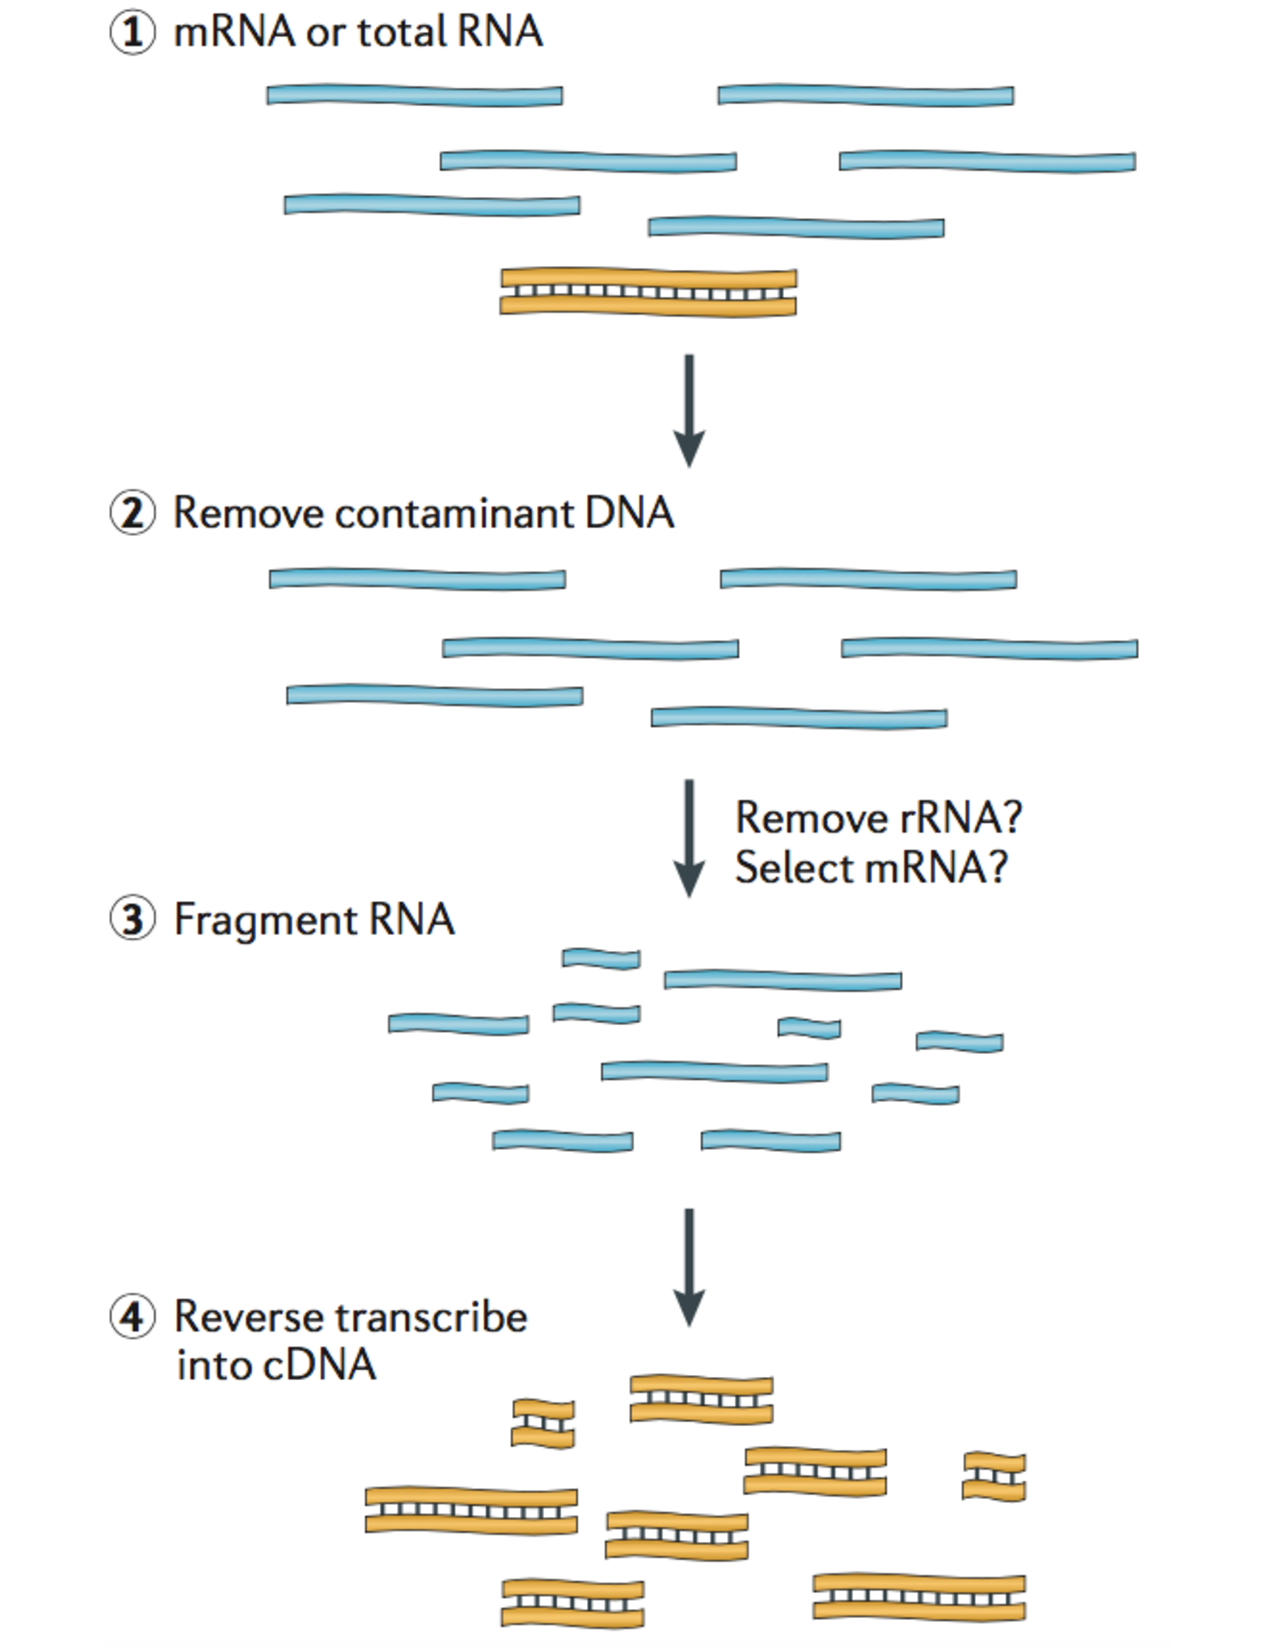
\includegraphics[width=\textwidth]{figures/seq1.pdf}
	\column{0.48\textwidth} 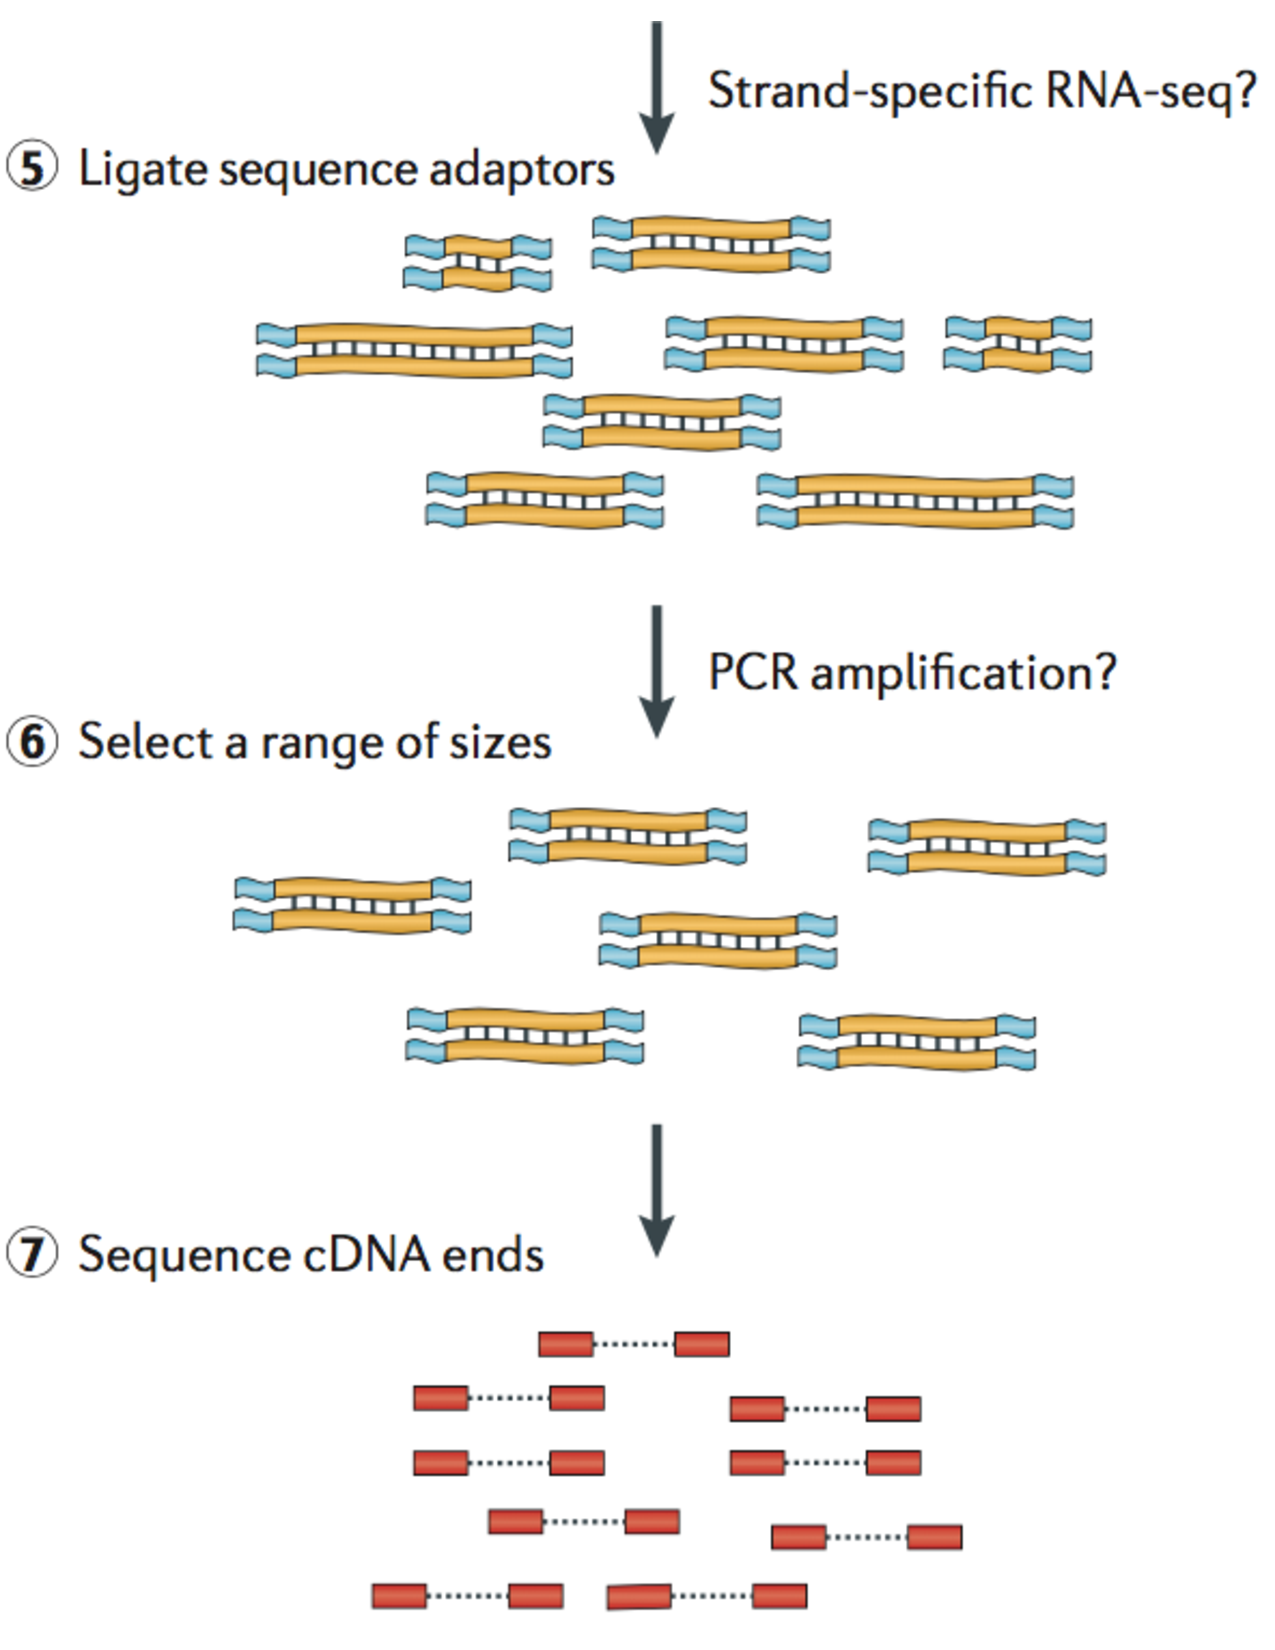
\includegraphics[width=\textwidth]{figures/seq2.pdf}
	\end{columns}

	\vspace{0.25cm}
	\onslide<2->{{\bf Computational Task:} Determine the transcripts and their abundance from the (paired-end) reads.}
}

\frame
{
	\frametitle{Splice Graph}
	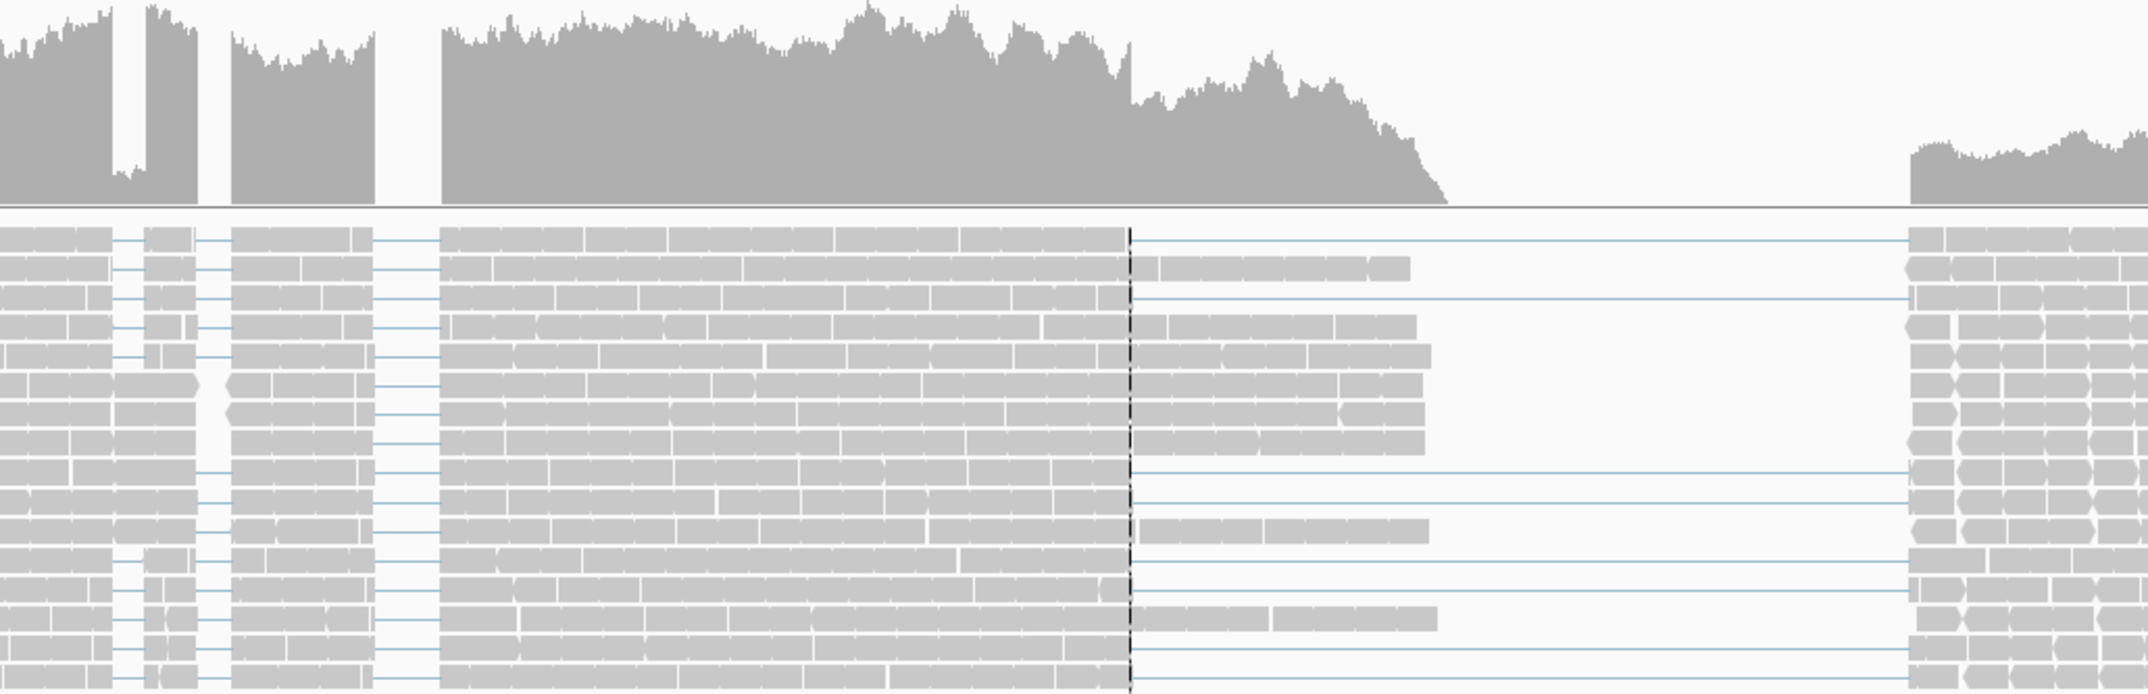
\includegraphics[width=\textwidth]{figures/reference.pdf}
	\vspace{0.2cm}
	\begin{center}

\begin{tikzpicture}[font=\small,overlay,
mycirclex/.style={draw, circle, minimum size=1.0em, inner sep = 0.2mm}, 
mydiamond/.style={draw, diamond, minimum size=0.78em, inner sep = 0mm}, 
myrectang/.style={draw, rectangle, minimum size=0.60em, inner sep = 0mm}, 
>=stealth]

\begin{scope}[xshift = -6cm, yshift=3.5cm]
\path<2-> node[blue] at (0.9cm, 0) {$1$};
\path<2-> node[blue] at (1.25cm, 0) {$2$};
\path<2-> node[blue] at (1.47cm,0) {$3$};
\path<2-> node[blue] at (2.1cm, 0) {$4$};
\path<2-> node[blue] at (4.5cm, 0) {$5$};
\path<2-> node[blue] at (7.0cm, 0) {$6$};
\path<2-> node[blue] at(10.8cm, 0) {$7$};
\end{scope}


\end{tikzpicture}
\end{center}

	\vspace{-0.4cm}
	\begin{center}

\begin{tikzpicture}[font=\small,overlay,
mycirclex/.style={draw, circle, minimum size=1.0em, inner sep = 0.2mm}, 
mydiamond/.style={draw, diamond, minimum size=0.78em, inner sep = 0mm}, 
myrectang/.style={draw, rectangle, minimum size=0.60em, inner sep = 0mm}, 
>=stealth]

\definecolor{mygreen}{rgb}{0, 0.7, 0}
\definecolor{myyellow}{rgb}{0.8, 0.6, 0}

\def\colx{black}
\def\cola{red} 
\def\colb{blue}
\def\colc{violet}
\def\cold{cyan} 
\def\cole{myyellow}
\def\colf{brown}


\def\len{2.0cm}

% G1
\begin{scope}[local bounding box=bbox, xshift=-6.0cm]
\path<1-> node[mycirclex] (v1) at (1.0 * \len, 0) {$s$};
\path<1-> node[mycirclex] (v2) at (2.0 * \len, 0) {$a$};
\path<1-> node[mycirclex] (v3) at (3.0 * \len, 0) {$b$};
\path<1-> node[mycirclex] (v4) at (4.0 * \len, 0) {$c$};
\path<1-> node[mycirclex] (v5) at (5.0 * \len, 0) {$t$};

\path<1-> [draw, \colx, ->, line width=0.04cm] (v1) -- (v2);
\path<1-> [draw, \colx, ->, line width=0.04cm] (v2) -- (v3);
\path<1-> [draw, \colx, ->, line width=0.04cm] (v3) -- (v4);
\path<1-> [draw, \colx, ->, line width=0.04cm] (v4) -- (v5);

\path<1-> [draw, \colx, ->, line width=0.04cm, bend left = 40] (v1) to (v3);
\path<1-> [draw, \colx, ->, line width=0.04cm, bend left = 40] (v3) to (v5);
\path<1-> [draw, \colx, ->, line width=0.04cm, bend left = 40] (v2) to (v4);

\path<1-> node at (1.5 * \len, 0.18cm) {$e_1(8)$};
\path<1-> node at (2.5 * \len, 0.18cm) {$e_2(2)$};
\path<1-> node at (3.5 * \len, 0.18cm) {$e_3(4)$};
\path<1-> node at (4.5 * \len, 0.18cm) {$e_4(10)$};

\path<1-> node at (2.0 * \len, 1.0cm) {$e_5(5)$};
\path<1-> node at (3.0 * \len, 1.0cm) {$e_6(6)$};
\path<1-> node at (4.0 * \len, 1.0cm) {$e_7(3)$};

\end{scope}
%\path<1-> [draw, rounded corners] ($(bbox.south west) - (0.00cm, 0.25cm)$) rectangle ($(bbox.north east) + (0.1cm, 0)$);
%\node at ($(bbox.south) - (0.00cm, 0.2cm)$) [label=below:{$G_2 - G_1 = \{c\}$}]{};


\end{tikzpicture}
\end{center}

	\vspace{0.2cm}
	\begin{itemize}
	\item<3-> {\bf Nodes:} continuous regions not seperated by spliced reads
	\item<3-> {\bf Edges:} adjacent regions or connected by spliced reads
	\item<3-> {\bf Weight of Nodes:} estimated from the average coverage
	\item<3-> {\bf Weight of Edges:} estimated from number of spliced reads
	\end{itemize}
}

\frame
{
	\frametitle{Optimization Problem}

	\begin{itemize}
	\item {\bf Input:} Directed acyclic graph~(DAG) $G=(V,E)$ with a single source $s$ and a single sink $t$;
		weight $w(e)$ for $e\in E$.

	\vspace{0.2cm}

	\item {\bf Output:} A set of paths $\mathcal{P}$ from $s$ to $t$ and abundance $a(P)$ for $P\in\mathcal{P}$, such that
		\begin{enumerate}
		\item each $e\in E$ is covered by at least one $P\in\mathcal{P}$, and that
		\item $|\mathcal{P}|$ is as small as possible, and that
		\item $\sum_{e\in E} \|w(e) - \sum_{e\in P} a(P)\|$ is as small as possible.
		\end{enumerate}
	\end{itemize}

	\vspace{1.0cm}
	\begin{center}

\begin{tikzpicture}[font=\small,overlay,
mycirclex/.style={draw, circle, minimum size=1.0em, inner sep = 0.2mm}, 
mydiamond/.style={draw, diamond, minimum size=0.78em, inner sep = 0mm}, 
myrectang/.style={draw, rectangle, minimum size=0.60em, inner sep = 0mm}, 
>=stealth]

\definecolor{mygreen}{rgb}{0, 0.7, 0}
\definecolor{myyellow}{rgb}{0.8, 0.6, 0}

\def\colx{black}
\def\cola{red} 
\def\colb{blue}
\def\colc{violet}
\def\cold{cyan} 
\def\cole{myyellow}
\def\colf{brown}


\def\len{3.0cm}

% G1
\begin{scope}[local bounding box=bbox, xshift=-8.0cm]
\path<1-> node[mycirclex] (v1) at (1.0 * \len, 0) {$s$};
\path<1-> node[mycirclex] (v2) at (2.0 * \len, 0) {$a$};
\path<1-> node[mycirclex] (v3) at (3.0 * \len, 0) {$b$};
\path<1-> node[mycirclex] (v4) at (4.0 * \len, 0) {$t$};

\path<1-> [draw, \colc, ->, line width=0.04cm] (v1) -- (v2);
\path<1-> [draw, \colc, ->, line width=0.10cm, bend left = 40] (v2) to (v3);
\path<1-> [draw, \colc, ->, line width=0.10cm, bend left = 40] (v3) to (v4);

\path<1-> [draw, \colb, ->, line width=0.04cm] (v2) -- (v3);
\path<1-> [draw, \colb, ->, line width=0.10cm, bend left = 40] (v1) to (v2);
\path<1-> [draw, \colb, ->, line width=0.04cm, bend left = 40] (v3) to (v4);

\path<1-> [draw, \cola, ->, line width=0.04cm] (v3) -- (v4);
\path<1-> [draw, \cola, ->, line width=0.04cm, bend left = 40] (v1) to (v2);
\path<1-> [draw, \cola, ->, line width=0.04cm, bend left = 40] (v2) to (v3);


%\path<1-> [draw, \colx, ->, line width=0.02cm] (v1) -- (v2);
%\path<1-> [draw, \colx, ->, line width=0.02cm] (v2) -- (v3);
%\path<1-> [draw, \colx, ->, line width=0.02cm] (v3) -- (v4);
%
%\path<1-> [draw, \colx, ->, line width=0.02cm, bend left = 40] (v1) to (v2);
%\path<1-> [draw, \colx, ->, line width=0.02cm, bend left = 40] (v2) to (v3);
%\path<1-> [draw, \colx, ->, line width=0.02cm, bend left = 40] (v3) to (v4);

\path<1-> node at (1.5 * \len, 0.18cm) {$e_2(4)$};
\path<1-> node at (2.5 * \len, 0.18cm) {$e_4(3)$};
\path<1-> node at (3.5 * \len, 0.18cm) {$e_6(2)$};

\path<1-> node at (1.5 * \len, 0.85cm) {$e_1(5)$};
\path<1-> node at (2.5 * \len, 0.85cm) {$e_3(6)$};
\path<1-> node at (3.5 * \len, 0.85cm) {$e_5(7)$};

\end{scope}
%\path<1-> [draw, rounded corners] ($(bbox.south west) - (0.00cm, 0.25cm)$) rectangle ($(bbox.north east) + (0.1cm, 0)$);
%\node at ($(bbox.south) - (0.00cm, 0.2cm)$) [label=below:{$G_2 - G_1 = \{c\}$}]{};


\end{tikzpicture}
\end{center}

	\vspace{1.0cm}
}

\frame
{
	\frametitle{Outline}
	\begin{enumerate}
	\item Algorithmic results
		\begin{itemize}
		\item Hardness results
		\item Polynomial-time algorithms
		\item Approximation algorithms
		\item Open problems
		\end{itemize}
	\item Existing Methods/Softwares
		\begin{itemize}
		\item Cufflinks
		\item Scripture
		\item IsoLasso
		\item Traph
		\item CLIIQ
		\item StringTie
		\end{itemize}
	\item Our initial thoughts
	\end{enumerate}
}


